\documentclass[UTF8,11pt,a4paper]{ctexart}

\usepackage{amsmath,amssymb,mathtools}
\usepackage{geometry}
\usepackage{enumitem}
\usepackage{graphicx}
\usepackage{float}
\usepackage{hyperref}
\usepackage{xcolor}

\geometry{top=2.2cm,bottom=2.2cm,left=2.4cm,right=2.4cm}
\hypersetup{colorlinks=true,linkcolor=blue!50!black}
\setlength{\parindent}{2em}
\setlength{\parskip}{0.25em}
\setlist[enumerate,1]{label=\arabic*.,leftmargin=2.6em,itemsep=0.65em,topsep=0.4em}
\setlist[enumerate,2]{label=(\arabic*),leftmargin=2.5em,itemsep=0.25em,topsep=0.2em}

\newcommand{\dd}{\,\mathrm{d}}
\newcommand{\ee}{\mathrm{e}}
\newcommand{\ii}{\mathrm{i}}
\newcommand{\Res}{\operatorname{Res}}
\newcommand{\Arg}{\operatorname{arg}}
\newcommand{\Ln}{\operatorname{Ln}}
\newcommand{\Ree}{\operatorname{Re}}
\newcommand{\Imm}{\operatorname{Im}}
\newcommand{\sh}{\operatorname{sh}}
\newcommand{\ch}{\operatorname{ch}}
\newcommand{\thh}{\operatorname{th}}

\title{\bfseries\Large 《复变函数与积分变换》习题汇编}
\author{据李江涛主编教材整理}
\date{}

\begin{document}
\maketitle

\begin{center}
\small
整理范围：习题一 P16--P17，习题二 P32--P33，习题三 P48--P50，习题四 P70--P73，
习题五 P87--P89，习题六 P108--P110，习题七 P128--P132，习题八 P147--P151。

正文按扫描页转录，并根据校对修正已确认的公式与文字错误。
\end{center}

\tableofcontents
\newpage

\section{习题一：复数与复变函数（P16--P17）}

\begin{enumerate}
\item 求下列复数的实部与虚部、共轭复数、模与辐角。
  \begin{enumerate}
  \item $\dfrac{1}{3+2\ii}$；
  \item $\dfrac{1}{\ii}-\dfrac{3\ii}{1-\ii}$；
  \item $\dfrac{(3+4\ii)(2-5\ii)}{2\ii}$；
  \item $\ii^8-4\ii^{21}+\ii$。
  \end{enumerate}

\item 如果等式
\[
\frac{x+1+\ii(y-3)}{5+3\ii}=1+\ii
\]
成立，试求实数 $x,y$ 为何值。

\item 试证虚数单位满足：$-\ii=\ii^{-1}$。

\item 求 $\dfrac{(3+4\ii)^2}{(1-2\ii)(3-\ii)}$ 的模。

\item 试证：
\[
|z_1+z_2|^2+|z_1-z_2|^2=2\bigl(|z_1|^2+|z_2|^2\bigr).
\]

\item 将下列复数化成三角表示式和指数表示式。
  \begin{enumerate}
  \item $\ii$；
  \item $-1$；
  \item $1+\sqrt{3}\ii$；
  \item $1-\cos\varphi+\ii\sin\varphi\ (0\leqslant\varphi\leqslant\pi)$；
  \item $\dfrac{2\ii}{-1+\ii}$；
  \item $\dfrac{(\cos5\varphi+\ii\sin5\varphi)^2}
  {(\cos3\varphi-\ii\sin3\varphi)^3}$。
  \end{enumerate}

\item 当 $|z|\leqslant1$ 时，求 $|z^n+a|$ 的最大值，其中 $n$ 为正整数，$a$ 为复数。

\item 一个复数乘以 $-\ii$，它的模与辐角有何改变？

\item 判断下列命题的真假。
  \begin{enumerate}
  \item 若 $c$ 为实数，则 $c=\overline c$；
  \item 若 $z$ 为纯虚数，则 $z\ne\overline z$；
  \item $2\ii<3\ii$；
  \item $\arg0=0$；
  \item 方程 $z=-\dfrac1z$ 仅有一个根；
  \item $\sqrt[3]{-1}=-1$；
  \item $\overline{\ii z}=\dfrac1\ii\,\overline z$。
  \end{enumerate}

\item 如果 $z=\ee^{\ii t}$，试证明
  \begin{enumerate}
  \item $z^n+\dfrac1{z^n}=2\cos nt$；
  \item $z^n-\dfrac1{z^n}=2\ii\sin nt$。
  \end{enumerate}

\item 求方程 $z^3+8=0$ 的所有根。

\item 求下列各式的值。
  \begin{enumerate}
  \item $(\sqrt3-\ii)^5$；
  \item $(1+\ii)^6$；
  \item $\sqrt[6]{-1}$；
  \item $(1-\ii)^{1/3}$。
  \end{enumerate}

\item 指出下列各题中点 $z$ 的存在范围，并作图。
  \begin{enumerate}
  \item $|z-\ii|=6$；
  \item $|z+2\ii|\geqslant1$；
  \item $\Ree z^2\leqslant1$；
  \item $\Ree(\ii z)=3$；
  \item $|z+\ii|=|z-\ii|$；
  \item $|z+3|+|z+1|=4$；
  \item $\left|\dfrac1z\right|<3$；
  \item $\left|\dfrac{z-3}{z-2}\right|\geqslant1$；
  \item $|\arg z|\leqslant\dfrac\pi3$；
  \item $\arg(z-\ii)=\dfrac\pi4$。
  \end{enumerate}

\item 描出下列不等式所确定的区域，并指出是有界的还是无界的、闭的还是开的、单连通的还是多连通的。
  \begin{enumerate}
  \item $\Imm z>0$；
  \item $|z-1|>4$；
  \item $0<\Ree z<1$；
  \item $1<|z-3\ii|<2$；
  \item $|z-1|<|z+3|$；
  \item $1<\arg z<1+\pi$；
  \item $|z-1|<4|z+1|$；
  \item $\dfrac12\leqslant\left|z-\dfrac12\right|\leqslant\dfrac32$；
  \item $|z|+\Ree z<1$；
  \item $z\overline z+(6+\ii)z+(6-\ii)\overline z\leqslant4$。
  \end{enumerate}

\item 证明复平面上的圆周方程可写为
\[
z\overline z+\alpha\overline z+\overline\alpha z+c=0
\]
（其中 $\alpha$ 为复常数，$c$ 为实常数）。

\item 画出下列方程（$t$ 是实参数）给出的曲线的图像。
  \begin{enumerate}
  \item $z=(1+\ii)t$；
  \item $z=a\cos t+\ii b\sin t$；
  \item $z=t+\dfrac\ii t$；
  \item $z=t^2+\dfrac\ii{t^2}$。
  \end{enumerate}

\item 函数 $w=\dfrac1z$ 将 $z$ 平面上的下列曲线变成 $w$ 平面上的什么曲线（$z=x+\ii y,w=u+\ii v$）？
  \begin{enumerate}
  \item $x^2+y^2=6$；
  \item $y=x$；
  \item $y=1$；
  \item $(x-1)^2+y^2=1$。
  \end{enumerate}

\item 试求
  \begin{enumerate}
  \item $\displaystyle\lim_{z\to1+\ii}\frac{\overline z}{z}$；
  \item $\displaystyle\lim_{z\to1}\frac{z\overline z+2z-\overline z-2}{z^2-1}$。
  \end{enumerate}

\item 试证 $\displaystyle\lim_{z\to0}\frac1{2\ii}\left(\frac z{\overline z}-\frac{\overline z}{z}\right)$ 不存在。

\item 试证 $\arg z\ (-\pi<\arg z\leqslant\pi)$ 在负实轴上（包括原点）不连续，除此而外在 $z$ 平面上处处连续。

\item 设函数 $f(z)$ 在 $z_0$ 处连续，且 $f(z_0)\ne0$，证明存在 $z_0$ 的邻域使 $f(z)\ne0$。

\item 如果 $f(z)$ 在点 $z_0$ 处连续，证明 $\overline{f(z)}$、$|f(z)|$ 也在点 $z_0$ 处连续。
\end{enumerate}

\newpage
\section{习题二：解析函数（P32--P33）}

\begin{enumerate}
\item 利用导数定义求函数 $f(z)=\dfrac1z$ 在 $z=1$ 处的导数。

\item 下列函数何处可导？何处解析？
  \begin{enumerate}
  \item $f(z)=x^2-\ii y$；
  \item $f(z)=xy^2+\ii x^2y$；
  \item $f(z)=\dfrac{x+y}{x^2+y^2}+\ii\dfrac{x-y}{x^2+y^2}$；
  \item $f(z)=\Imm z$。
  \end{enumerate}

\item 试确定下列函数的解析区域和奇点，并求出导数。
  \begin{enumerate}
  \item $f(z)=(z-1)^2(z^2+3)$；
  \item $f(z)=z^3+2\ii z$；
  \item $f(z)=\dfrac1{z^2-1}$；
  \item $f(z)=\dfrac{2z+1}{z^3+1}$。
  \end{enumerate}

\item 试证下列函数在 $z$ 平面上任何点都不解析。
  \begin{enumerate}
  \item $f(z)=x+\ii2y$；
  \item $f(z)=x+y$；
  \item $f(z)=\Ree z$；
  \item $f(z)=\dfrac1{|\overline z|}$。
  \end{enumerate}

\item 若 $f(z)$ 在区域 $D$ 内解析，试证 $f(z)$ 在区域 $D$ 内连续。

\item 判断下述命题的真假，若真，请给出证明；若假，请举例说明。
  \begin{enumerate}
  \item 如果 $f'(z_0)$ 存在，那么 $f(z)$ 在 $z_0$ 点解析；
  \item 如果 $f(z)$ 在 $z_0$ 点连续，那么 $f'(z_0)$ 存在；
  \item 实部与虚部满足柯西--黎曼方程的复变函数是解析函数；
  \item 如果 $z_0$ 是 $f(z)$ 和 $g(z)$ 的一个奇点，则 $z_0$ 是 $f(z)+g(z)$ 和 $\dfrac{f(z)}{g(z)}$ 的一个奇点；
  \item 如果 $u(x,y)$ 和 $v(x,y)$ 的偏导数均存在，则 $f(z)=u(x,y)+\ii v(x,y)$ 的导数一定存在。
  \end{enumerate}

\item 证明：如果函数 $f(z)=u+\ii v$ 在区域 $D$ 内解析，并满足下列条件之一，那么 $f(z)$ 是常数。
  \begin{enumerate}
  \item $f(z)$ 恒取实值；
  \item $\overline{f(z)}$ 在 $D$ 内解析；
  \item $\arg f(z)$ 在 $D$ 内是一个常数；
  \item $au+bv=c$，其中 $a,b,c$ 为不全为零的实常数；
  \item $v=u^2$。
  \end{enumerate}

\item 设 $f(z)=my^3+nx^2y+\ii(x^3+lxy^2)$ 在全平面上解析，试确定 $l,m,n$ 的值。

\item 如果 $f(z)=u(x,y)+\ii v(x,y)$ 在区域 $D$ 内解析，试证：
\[
\left(\frac{\partial}{\partial x}|f(z)|\right)^2+
\left(\frac{\partial}{\partial y}|f(z)|\right)^2=|f'(z)|^2.
\]

\item 判断下列关系是否正确？
  \begin{enumerate}
  \item $\overline{\ee^z}=\ee^{\overline z}$；
  \item $\overline{\cos z}=\cos\overline z$；
  \item $\overline{\sin z}=\sin\overline z$；
  \item $|\sin z|\leqslant1$；
  \item $\ee^{z+2k\pi}=\ee^z\ (k=0,\pm1,\pm2,\ldots)$；
  \item $\ee^z>0$。
  \end{enumerate}

\item 找出下列方程的全部解。
  \begin{enumerate}
  \item $\sin z=0$；
  \item $\cos z=0$；
  \item $\cos z+\sin z=0$；
  \item $1+\ee^z=0$；
  \item $\sin z=\ch4$。
  \end{enumerate}

\item 证明。
  \begin{enumerate}
  \item $\cos(z_1+z_2)=\cos z_1\cos z_2-\sin z_1\sin z_2$，
  $\sin(z_1+z_2)=\sin z_1\cos z_2+\cos z_1\sin z_2$；
  \item $\sin^2z+\cos^2z=1$；
  \item $\sin2z=2\sin z\cos z$；
  \item $\tan2z=\dfrac{2\tan z}{1-\tan^2z}$；
  \item $\sin\left(\dfrac\pi2-z\right)=\cos z$；
  \item $\cos(z+\pi)=-\cos z$。
  \end{enumerate}

\item 化简。
  \begin{enumerate}
  \item $\ee^{1+\pi\ii}+\cos\ii$；
  \item $\ch\dfrac\pi4\ii$；
  \item $\cos(\ii\ln5)$。
  \end{enumerate}

\item 已知
\[
f(z)=\frac{\ln\left(\dfrac12+z^2\right)}
{\sin\left(\dfrac{1+\ii}{4}\pi z\right)},
\]
求 $|f'(1-\ii)|$ 及 $\arg f'(1-\ii)$。

\item 求 $\Ln(-\ii)$、$\Ln(-3+4\ii)$ 的值及其主值。

\item 求 $\ee^{1-\ii\pi/2}$、$3^{\ii}$ 和 $(1+\ii)^{\ii}$ 的值。

\item 解下列方程：
  \begin{enumerate}
  \item $\ln z=2-\ii\dfrac\pi6$；
  \item $\sh z=\ii$。
  \end{enumerate}

\item 指出下列运算中的错误所在。
  \begin{enumerate}
  \item $1=\sqrt1=\sqrt{(-1)(-1)}=\sqrt{-1}\sqrt{-1}=-1$；
  \item
  \[
  \begin{aligned}
  \frac\pi4&=\arctan1=\int_0^1\frac{\dd x}{1+x^2}
  =\frac1{2\ii}\int_0^1\left(-\frac1{\ii-x}-\frac1{x+\ii}\right)\dd x\\
  &=\left.\frac1{2\ii}\Ln\frac{\ii-x}{\ii+x}\right|_{x=0}^{x=1}
  =\frac1{2\ii}\Ln\frac{\ii-1}{\ii+1}
  =\frac1{8\ii}\Ln\left(\frac{\ii-1}{\ii+1}\right)^4
  =\frac1{8\ii}\Ln1=0.
  \end{aligned}
  \]
  \end{enumerate}
\end{enumerate}

\newpage
\section{习题三：复变函数的积分（P48--P50）}

\begin{enumerate}
\item 沿下列路线计算积分 $\displaystyle\int_0^{3+\ii}z^2\dd z$。
  \begin{enumerate}
  \item 自原点到 $3+\ii$ 的直线段；
  \item 自原点沿实轴至 $3$，再由 $3$ 沿垂直向上至 $3+\ii$；
  \item 自原点沿虚轴至 $\ii$，再由 $\ii$ 沿水平方向右至 $3+\ii$。
  \end{enumerate}

\item 分别沿 $y=x$ 与 $y=x^2$ 算出积分
$\displaystyle\int_0^{1+\ii}(x^2+\ii y)\dd z$ 的值。

\item 计算积分 $\displaystyle\oint_C|z|\overline z\dd z$，其中 $C$ 是一条闭路，由直线段 $-1\leqslant x\leqslant1,y=0$ 与上半单位圆周组成。

\item 证明下列不等式。
  \begin{enumerate}
  \item $\displaystyle\left|\int_C(x^2+\ii y^2)\dd z\right|\leqslant2$，其中 $C$ 是从 $-\ii$ 到 $\ii$ 的直线段；
  \item $\displaystyle\left|\int_C(x^2+\ii y^2)\dd z\right|\leqslant\pi$，其中 $C$ 是从 $-\ii$ 到 $\ii$ 的右半圆周。
  \end{enumerate}

\item 设 $f(z)$ 在单连通区域 $D$ 内解析，$C$ 为 $D$ 内任何一条正向简单闭曲线，问
\[
\oint_C\Ree[f(z)]\dd z=\oint_C\Imm[f(z)]\dd z=0
\]
是否成立？如果成立，给出证明；如果不成立，举例说明。

\item 利用在单位圆上 $\overline z=\dfrac1z$ 的性质及柯西积分公式说明
$\displaystyle\oint_C\overline z\dd z=2\pi\ii$，其中 $C$ 表明单位圆周 $|z|=1$，且沿正向积分。

\item 计算积分 $\displaystyle\oint_C\dfrac{\overline z}{|z|}\dd z$ 的值，其中 $C$ 为正向圆周：
  \begin{enumerate}
  \item $|z|=2$；
  \item $|z|=4$。
  \end{enumerate}

\item 直接得到下列积分的结果，并说明理由。
  \begin{enumerate}
  \item $\displaystyle\oint_{|z|=1}\frac{3z+5}{z^2+2z+4}\dd z$；
  \item $\displaystyle\oint_{|z|=1}\frac{\ee^z}{\cos z}\dd z$；
  \item $\displaystyle\oint_{|z|=2}\ee^z(z^2+1)\dd z$；
  \item $\displaystyle\oint_{|z|=1/2}\frac{\dd z}{(z^2-1)(z^3-1)}$。
  \end{enumerate}

\item 沿指定曲线的正向计算下列各积分。
  \begin{enumerate}
  \item $\displaystyle\oint_C\frac{\ee^z}{z-2}\dd z,\quad C:|z-2|=1$；
  \item $\displaystyle\oint_C\frac{\cos\pi z}{(z-1)^5}\dd z,\quad C:|z|=r>1$；
  \item $\displaystyle\oint_C\frac{\sin z}{(z-\pi/2)^2}\dd z,\quad C:|z|=2$；
  \item $\displaystyle\oint_C\frac{\dd z}{(z^2+1)(z^2+4)},\quad C:|z|=\dfrac32$；
  \item $\displaystyle\oint_C\frac{3z^2+7z+1}{(z+1)^3}\dd z,\quad C:|z+\ii|=1$；
  \item $\displaystyle\oint_C\frac{\dd z}{z^2-a^2},\quad C:|z-a|=a\quad(a>0)$；
  \item $\displaystyle\oint_C\frac{\cos z}{z^3}\dd z$，其中 $C=C_1+C_2$，$C_1:|z|=2$，$C_2:|z|=3$；
  \item $\displaystyle\oint_C\frac{\ee^z}{(z-a)^3}\dd z$，其中 $a$ 为 $|a|\ne1$ 的任何复数，$C:|z|=1$；
  \item $\displaystyle\oint_C\frac{\ee^z\sin z}{z^2}\dd z,\quad C:|z-\ii|=2$；
  \item $\displaystyle\oint_C\frac{3z+2}{z^4-1}\dd z,\quad C:|z-(1+\ii)|=\sqrt2$。
  \end{enumerate}

\item 设 $C$ 为不经过 $a$ 与 $-a$ 的正向简单闭曲线，$a$ 为不等于零的任何复数，试就 $a$ 与 $-a$ 同 $C$ 的各种不同位置，计算积分
$\displaystyle\oint_C\frac{z}{z^2-a^2}\dd z$。

\item 设 $f(z)$ 与 $g(z)$ 在区域 $D$ 内处处解析，$C$ 为 $D$ 内任何一条简单光滑闭曲线，它的内部全属于 $D$。如果 $f(z)=g(z)$ 在 $C$ 上所有点都成立，试证在 $C$ 的内部所有点处 $f(z)=g(z)$ 也成立。

\item 验证下列函数是调和函数，并求出以 $z=x+\ii y$ 为自变量的解析函数 $w=f(z)=u+\ii v$。
  \begin{enumerate}
  \item $v=\arctan\dfrac yx\quad(x>0)$；
  \item $u=\ee^x(y\cos y+x\sin y)+x+y,\quad f(0)=\ii$；
  \item $u=(x-y)(x^2+4xy+y^2)$；
  \item $v=\dfrac{y}{x^2+y^2},\quad f(2)=0$。
  \end{enumerate}

\item 设 $u$ 为区域 $D$ 中的调和函数及
$f(z)=\dfrac{\partial u}{\partial x}-\ii\dfrac{\partial u}{\partial y}$，$f$ 是不是 $D$ 内解析函数？为什么？

\item 函数 $v=x+y$ 是 $u=x+y$ 的共轭调和函数吗？为什么？

\item 如果 $f(z)=u+\ii v$ 是一解析函数，试证：
  \begin{enumerate}
  \item $\overline{\ii\,\overline{f(z)}}$ 也是解析函数；
  \item $-u$ 是 $v$ 的共轭调和函数。
  \end{enumerate}

\item 证明 $u=x^2-y^2$ 和 $v=\dfrac{y}{x^2+y^2}$ 都是调和函数，但 $u+\ii v$ 不是解析函数。

\item 如果 $f(z)=u+\ii v$ 是 $z$ 的解析函数，证明
\[
\left(\frac{\partial^2}{\partial x^2}+\frac{\partial^2}{\partial y^2}\right)|f(z)|^2
=4|f'(z)|^2.
\]

\item 证明：若 $f(z)$ 在单位圆 $|z|<1$ 内解析，$|f(z)|\leqslant\dfrac1{1-|z|}$，则
\[
|f^{(n)}(0)|<\ee(n+1)!,\qquad n=1,2,\ldots.
\]

\item 设 $f(z)$ 在单连通区域 $D$ 内解析，且不为零，$C$ 为 $D$ 内任何一条简单光滑闭曲线，问积分
$\displaystyle\oint_C\dfrac{f'(z)}{f(z)}\dd z$ 是否为零？为什么？
\end{enumerate}

\newpage
\section{习题四：解析函数的级数展开及其应用（P70--P73）}

\begin{enumerate}
\item 讨论下列数列的敛散性，如果收敛，求出它们的极限。
  \begin{enumerate}
  \item $a_n=\dfrac{1+n\ii}{1-n\ii}$；
  \item $a_n=\left(1+\dfrac\ii2\right)^{-n}$；
  \item $a_n=(-1)^n+\dfrac\ii{n+1}$；
  \item $a_n=\dfrac1n\ee^{-n\pi\ii/2}$。
  \end{enumerate}

\item 判断下列级数敛散性。
  \begin{enumerate}
  \item $\displaystyle\sum_{n=1}^{\infty}\frac{\ii^n}{n}$；
  \item $\displaystyle\sum_{n=2}^{\infty}\frac{\ii^n}{\ln n}$；
  \item $\displaystyle\sum_{n=1}^{\infty}\frac{(6+5\ii)^n}{8^n}$；
  \item $\displaystyle\sum_{n=1}^{\infty}\frac{\cos(\ii n)}{2^n}$。
  \end{enumerate}

\item 求下列级数的收敛半径。
  \begin{enumerate}
  \item $\displaystyle\sum_{n=0}^{\infty}\frac n{2^n}z^n$；
  \item $\displaystyle\sum_{n=0}^{\infty}\frac{z^n}{n!}$；
  \item $\displaystyle\sum_{n=1}^{\infty}\frac{n!}{n^n}z^n$。
  \end{enumerate}

\item 下列结论是否正确？为什么？
  \begin{enumerate}
  \item 每一个幂级数在它的收敛圆内与收敛圆上收敛；
  \item 每一个幂级数收敛于一个解析函数；
  \item 每一个在 $z_0$ 连续的函数一定可以在 $z_0$ 的邻域内展开成 Taylor 级数。
  \end{enumerate}

\item 幂级数 $\displaystyle\sum_{n=0}^{\infty}a_n(z-2)^n$ 能否在 $z=0$ 收敛而在 $z=3$ 发散？

\item 如果 $\displaystyle\sum_{n=0}^{\infty}a_nz^n$ 的收敛半径为 $R$，证明级数
$\displaystyle\sum_{n=0}^{\infty}(\Ree a_n)z^n$ 的收敛半径 $\geqslant R$。

\item 函数 $\dfrac1{1+x^2}$ 当 $x$ 为任何实数时都有确定的值，但它的 Taylor 展开式
\[
\frac1{1+x^2}=1-x^2+x^4+\cdots
\]
却只当 $|x|<1$ 时成立，试说明其原因。

\item 把下列各函数展开成 $z$ 的幂级数，并指出它们的收敛半径。
  \begin{enumerate}
  \item $\dfrac1{1+z^3}$；
  \item $\dfrac1{(1+z^2)^2}$；
  \item $\cos z^2$；
  \item $\sh z$；
  \item $\ee^{z^2}\sin z^2$；
  \item $\sin\dfrac1{1-z}$。
  \end{enumerate}

\item 求下列函数在指定点 $z_0$ 处的 Taylor 展开式，并指出它们的收敛半径。
  \begin{enumerate}
  \item $\dfrac{z-1}{z+1},\ z_0=1$；
  \item $\dfrac z{(z+1)(z+2)},\ z_0=2$；
  \item $\dfrac1{z^2},\ z_0=-1$；
  \item $\dfrac1{4-3z},\ z_0=1+\ii$；
  \item $f(z)=\displaystyle\int_0^z\ee^{\xi^2}\dd\xi,\ z_0=0$；
  \item $\sin(2z-z^2),\ z_0=1$；
  \item $\ee^{z\ln(1+z)},\ z_0=0$；
  \item $[\ln(1+z)]^2,\ z_0=0$；
  \item $\ln z,\ z_0=\ii$；
  \item $\ee^{1/(1-z)},\ z_0=0$。
  \end{enumerate}

\item 把下列各函数在指定的圆环域内展开成 Laurent 级数。
  \begin{enumerate}
  \item $\dfrac1{(z^2+1)(z-2)},\ 1<|z|<2$；
  \item $\dfrac1{z(1-z)^2},\ 0<|z|<1,\ 0<|z-1|<1$；
  \item $\dfrac1{(z-1)(z-2)},\ 0<|z-1|<1,\ 1<|z-2|<+\infty$；
  \item $\ee^{1/(1-z)},\ 1<|z|<+\infty$；
  \item $\sin\dfrac1{1-z},\ 0<|z-1|<+\infty$；
  \item $\dfrac1{z(\ii-z)},\ 0<|z-\ii|<1$；
  \item $\dfrac{z^2-2z+5}{(z-2)(z^2+1)},\ 1<|z|<2,\ 2<|z|<+\infty$；
  \item $\dfrac1{z(z+2)^3},\ 0<|z|<1$；
  \item $\dfrac{\ee^z}{z(z^2+1)},\ 0<|z|<1$。
  \end{enumerate}

\item 问下列各函数有哪些孤立奇点？各属于哪一种类型？如果是极点，指出它的级。
  \begin{enumerate}
  \item $\dfrac1{z^3(z^2+1)^2}$；
  \item $\dfrac{\ee^z\sin z}{z^2}$；
  \item $\dfrac1{z^3-z^2-z+1}$；
  \item $\dfrac1{\sin z}$；
  \item $\dfrac z{(1+z^2)(1+\ee^z)}$；
  \item $\sin\dfrac1{1-z}$；
  \item $\ee^{z-1/z}$；
  \item $\sin\dfrac1z+\dfrac1{z^2}$；
  \item $\ee^{z/(1-z)}$；
  \item $\dfrac{z^{2n}}{1+z^n}$；
  \item $\dfrac{\ln(z+1)}z$；
  \item $\dfrac{\ee^{1/(1-z)}}{\ee^z-1}$。
  \end{enumerate}

\item 指出下列函数在无穷远点的性质。
  \begin{enumerate}
  \item $\dfrac1{z-z^3}$；
  \item $\dfrac{z^4}{1+z^4}$；
  \item $\dfrac{z^6}{(z^2-3)^2\cos\dfrac1{z-2}}$；
  \item $\dfrac1{\ee^z-1}-\dfrac1z$；
  \item $\dfrac{\ee^z}{z(1-\ee^{-z})}$；
  \item $\ee^{-z}\cos\dfrac1z$。
  \end{enumerate}

\item 若 $f(z)$ 与 $g(z)$ 分别以 $z=z_0$ 为 $m$ 级与 $n$ 级极点，试问下列函数在 $z=z_0$ 点有何性质？
  \begin{enumerate}
  \item $f(z)+g(z)$；
  \item $f(z)g(z)$；
  \item $\dfrac{f(z)}{g(z)}$。
  \end{enumerate}

\item 若 $f(z)$ 在 $z_0$ 点解析，$g(z)$ 在 $z_0$ 点有本性奇点，试问：
  \begin{enumerate}
  \item $f(z)+g(z)$；
  \item $f(z)g(z)$；
  \item $\dfrac{f(z)}{g(z)}$ 在 $z_0$ 有何性质？
  \end{enumerate}

\item 求证：如果 $z_0$ 是 $f(z)$ 的 $m\ (m\geqslant2)$ 级零点，那么 $z_0$ 是 $f'(z)$ 的 $m-1$ 级零点。

\item 函数 $f(z)=\dfrac1{(z-1)(z-2)^3}$ 在 $z=2$ 处有一个三级极点，这个函数又有如下的 Laurent 展开式
\[
\frac1{(z-1)(z-2)^3}=\cdots+\frac1{(z-2)^6}-\frac1{(z-2)^5}+\frac1{(z-2)^4},\qquad |z-2|>1.
\]
所以“$z=2$ 又是 $f(z)$ 的一个本性奇点”；又因为上式不含有 $(z-2)^{-1}$ 项，因此
$\Res[f(z),2]=0$。这些结论对否？

\item 设幂级数 $\displaystyle\sum_{n=0}^{\infty}a_nz^n$ 的收敛半径 $R>0$，和函数为 $f(z)$，证明：
\[
|a_n|\leqslant\frac{M(r)}{r^n},\qquad n=0,1,2,\ldots,
\]
其中 $0<r<R$，$M(r)=\displaystyle\max_{0\leqslant\theta\leqslant2\pi}|f(r\ee^{\ii\theta})|$。

\item 求证如下不等式。
  \begin{enumerate}
  \item 对任意的复数 $z$ 有 $|\ee^z-1|\leqslant\ee^{|z|}-1\leqslant|z|\ee^{|z|}$；
  \item 当 $0<|z|<1$ 时，证 $\dfrac14|z|<|\ee^z-1|<\dfrac74|z|$。
  \end{enumerate}

\item 设 $f(z)=\dfrac{z-a}{z+a},a\ne0$，求
$\displaystyle\oint_C\dfrac{f(z)}{z^{n+1}}\dd z$，其中 $C$ 为任一条包含原点且落在圆周 $|z|=|a|$ 内的简单闭曲线。

\item 讨论下列各函数在扩充复平面上有哪些孤立奇点？各属于哪一种类型？如果是极点，请指出它的级。
  \begin{enumerate}
  \item $\sin\dfrac z{z+1}$；
  \item $\ee^{z+1/z}$；
  \item $\sin z\cdot\sin\dfrac1z$；
  \item $\dfrac{\sh z}{\ch z}$；
  \item $\sin\left(\dfrac1{\sin(1/z)}\right)$；
  \item $\tan^2z$；
  \item $\dfrac1{\sin z-\sin a}$；
  \item $\ee^{\tan(1/z)}$。
  \end{enumerate}

\item 假设解析函数 $f(z)$ 在 $z_0$ 点有 $m$ 级零点，试问函数
$\displaystyle F(z)=\int_{z_0}^z f(\xi)\dd\xi$ 在点 $z_0$ 的性质如何？
\end{enumerate}
\section{习题五：留数及其应用（P87--P89）}

\begin{enumerate}
\item 求下列各函数 $f(z)$ 在孤立奇点的留数（不考虑无穷远点）。
  \begin{enumerate}
  \item $\dfrac1{z^3-z^5}$；
  \item $\dfrac{z^2}{(1+z^2)^2}$；
  \item $\dfrac{z^{2n}}{1+z^n}$（$n$ 为自然数）；
  \item $\dfrac{1-\ee^{2z}}{z^4}$；
  \item $\dfrac1{\sin z}$；
  \item $\tan z$。
  \end{enumerate}

\item 计算下列各积分（利用留数）。
  \begin{enumerate}
  \item $\displaystyle\oint_C\frac{z\dd z}{(z-1)(z-2)^2},\quad C:|z-2|=\frac12$；
  \item $\displaystyle\oint_C\frac{\dd z}{1+z^4},\quad C:x^2+y^2=2x$；
  \item $\displaystyle\oint_C\frac{\sin z}{z}\dd z,\quad C:|z|=\frac32$；
  \item $\displaystyle\oint_C\frac{3z^3+2}{(z-1)(z^2+9)}\dd z,\quad C:|z|=4$；
  \item $\displaystyle\oint_C\frac{\ee^{2z}}{(z-1)^2}\dd z,\quad C:|z|=2$；
  \item $\displaystyle\oint_C\frac{1-\cos z}{z^m}\dd z,\quad C:|z|=\frac32$，$m$ 为整数。
  \end{enumerate}

\item 求 $\Res[f(z),\infty]$ 的值，如果
  \begin{enumerate}
  \item $f(z)=\dfrac{\ee^z}{z^2-1}$；
  \item $f(z)=\dfrac1{z(z+1)^4(z-4)}$；
  \item $f(z)=\dfrac{2z}{3+z^2}$。
  \end{enumerate}

\item 设函数 $f(z)$ 在 $z=\infty$ 有可去奇点，求 $\Res[f^2(z),\infty]$。

\item 计算下列各积分，$C$ 为正向圆周。
  \begin{enumerate}
  \item $\displaystyle\oint_C\frac{\dd z}{z^3(z^{10}-2)},\quad C:|z|=2$；
  \item $\displaystyle\oint_C\frac{z^3}{1+z}\ee^{1/z}\dd z,\quad C:|z|=2$；
  \item $\displaystyle\frac1{2\pi\ii}\oint_C\frac{\ee^{zt}}{1+z^2}\dd z,\quad C:|z|=2$；
  \item $\displaystyle\oint_C\tan(\pi z)\dd z,\quad C:|z|=n$；
  \item $\displaystyle\oint_C z^n\ee^{2/z}\dd z,\quad C:|z|=r$，$n$ 为整数；
  \item $\displaystyle\oint_C\thh z\dd z,\quad C:|z-2\ii|=1$。
  \end{enumerate}

\item 试求下列各积分的值。
  \begin{enumerate}
  \item $\displaystyle\int_0^{2\pi}\frac{\dd\theta}{a+\cos\theta}\quad(a>1)$；
  \item $\displaystyle\int_0^\pi\frac{\cos2\theta}{1-2a\cos\theta+a^2}\dd\theta\quad(a^2<1)$；
  \item $\displaystyle\int_{-\infty}^{\infty}\frac{\dd x}{x^2+2x+2}$；
  \item $\displaystyle\int_{-\infty}^{\infty}\frac{x\dd x}{(1+x^2)(x^2+2x+2)}$；
  \item $\displaystyle\int_0^{+\infty}\frac{x\sin x}{1+x^2}\dd x$；
  \item $\displaystyle\int_{-\infty}^{\infty}\frac{(1+x^2)\cos ux}{1+x^2+x^4}\dd x$；
  \item $\displaystyle\int_0^{\infty}\frac{\sin x}{x(1+x^2)}\dd x$；
  \item $\displaystyle\int_0^\pi\frac{\dd\theta}{a^2+\sin^2\theta}\quad(a>0)$；
  \item $\displaystyle\int_{-\infty}^{\infty}\frac{\dd x}{(x^2+a^2)(x^2+b^2)}\quad(a>0,b>0)$；
  \item $\displaystyle\int_0^{\infty}\frac{\cos x}{(x^2+a^2)(x^2+b^2)}\dd x\quad(a>0,b>0)$；
  \item $\displaystyle\int_0^{\infty}\frac{x^2-b^2}{x^2+b^2}\cdot\frac{\sin ax}{x}\dd x\quad(a>0)$。
  \end{enumerate}

\item 设 $f(z)$ 在 $z$ 平面上解析，$f(z)=\displaystyle\sum_{n=0}^{\infty}a_nz^n$，则对任一正整数 $k$，求
$\displaystyle\Res\left[\frac{f(z)}{z^k},0\right]$。

\item 若 $f(z)$ 和 $g(z)$ 在点 $z_0$ 处解析，而且 $f(z_0)\ne0$，$g(z)$ 以 $z_0$ 为二级零点，证明：
\[
\Res\left[\frac{f(z)}{g(z)},z_0\right]
=\frac{a_1b_2-a_0b_3}{b_2^2},
\qquad a_k=\frac1{k!}f^{(k)}(z_0),\quad b_k=\frac1{k!}g^{(k)}(z_0).
\]

\item 若 $f(z)$ 在 $|z|\leqslant1$ 上解析且 $|f(z)|<1$，试问方程 $f(z)=z$ 在 $|z|<1$ 内有几个根。

\item 试证明若在简单闭曲线 $C$ 上有
\[
|a_kz^k|>|a_0+a_1z+\cdots+a_{k-1}z^{k-1}+a_{k+1}z^{k+1}+\cdots+a_nz^n|,
\]
则当 $z=0$ 位于 $C$ 内时，多项式 $a_0+a_1z+\cdots+a_nz^n$ 在 $C$ 内有 $k$ 个零点；又问当 $z=0$ 位于 $C$ 的外部时，将有什么结论？

\item 证明方程 $z^7-z^3+12=0$ 的根都在圆环域 $1\leqslant|z|\leqslant2$ 内。

\item 证明若 $|a|>\ee$，则方程 $\ee^z=az^n$ 在圆 $|z|<1$ 内有 $n$ 个根。

\item 若 $|a_k|<1\ (k=1,2,\ldots,n)$，$|b|<1$，且
\[
f(z)=\prod_{k=1}^{n}\left(\frac{z-a_k}{1-\overline{a_k}z}\right),
\]
则方程 $f(z)=b$ 在圆 $|z|<1$ 内有 $n$ 个根；若 $|b|>1$，则方程 $f(z)=b$ 在圆 $|z|\leqslant1$ 以外的区域恰有 $n$ 个根。
\end{enumerate}

\newpage
\section{习题六：共形映射（P108--P110）}

\begin{enumerate}
\item 求 $w=3z^2$ 在 $z=\ii$ 处的伸缩率和旋转角，问 $w=3z^2$ 将经过点 $z=\ii$ 且平行于实轴正向的曲线的切线方向映射成 $w$ 平面上哪一个方向？并作图。

\item 求映射 $w=\ii z$ 下，下列图形映射成什么图形？
  \begin{enumerate}
  \item 以 $z_1=\ii,z_2=-1,z_3=1$ 为顶点的三角形；
  \item 闭圆域：$|z-1|\leqslant1$。
  \end{enumerate}

\item 证明映射 $w=z+\dfrac1z$ 把圆周 $|z|=c\ (c>0)$ 映射成椭圆：
\[
u=\left(c+\frac1c\right)\cos\theta,\qquad
v=\left(c-\frac1c\right)\sin\theta.
\]

\item 证明在映射 $w=\ee^{\ii z}$ 下，互相正交的直线簇 $\Ree z=c_1$ 与 $\Imm z=c_2$ 依次映射成互相正交的直线簇
$v=u\tan c_1$ 与圆簇 $u^2+v^2=\ee^{-2c_2}$。

\item 映射 $w=z^2$ 把上半个圆域 $|z|<R,\Imm z>0$ 映射成什么？

\item 求下列区域在指定的映射下的像域。
  \begin{enumerate}
  \item $\Ree z>0,\quad w=\ii z+\ii$；
  \item $\Imm z>0,\quad w=(1+\ii)z$；
  \item $0<\Imm z<\dfrac12,\quad w=\dfrac1z$；
  \item $\Ree z>1,\Imm z>0,\quad w=\dfrac1z$。
  \end{enumerate}

\item 求把上半平面 $\Imm z>0$ 映射为单位圆 $|w|<1$ 的分式线性映射 $w=f(z)$，并满足条件：
  \begin{enumerate}
  \item $f(\ii)=0,f(-1)=1$；
  \item $f(\ii)=0,\arg f'(\ii)=0$。
  \end{enumerate}

\item 求把单位圆映射成单位圆的分式线性映射，并满足条件：
  \begin{enumerate}
  \item $f\left(\dfrac12\right)=0,f(-1)=1$；
  \item $f\left(\dfrac12\right)=0,\arg f'\left(\dfrac12\right)=\dfrac\pi2$。
  \end{enumerate}

\item 把点 $z=1,\ii,-\ii$ 分别映射成点 $w=1,0,-1$ 的分式线性映射把单位圆 $|z|<1$ 映射成什么？并求出这个映射。

\item 把图~\ref{fig:625} 阴影部分所示（边界为直线段或圆弧）的域 $D$ 保形地且互为单值地映射成上半平面 $G$，求出实现各该映射的任一函数。

\begin{figure}[H]
\centering
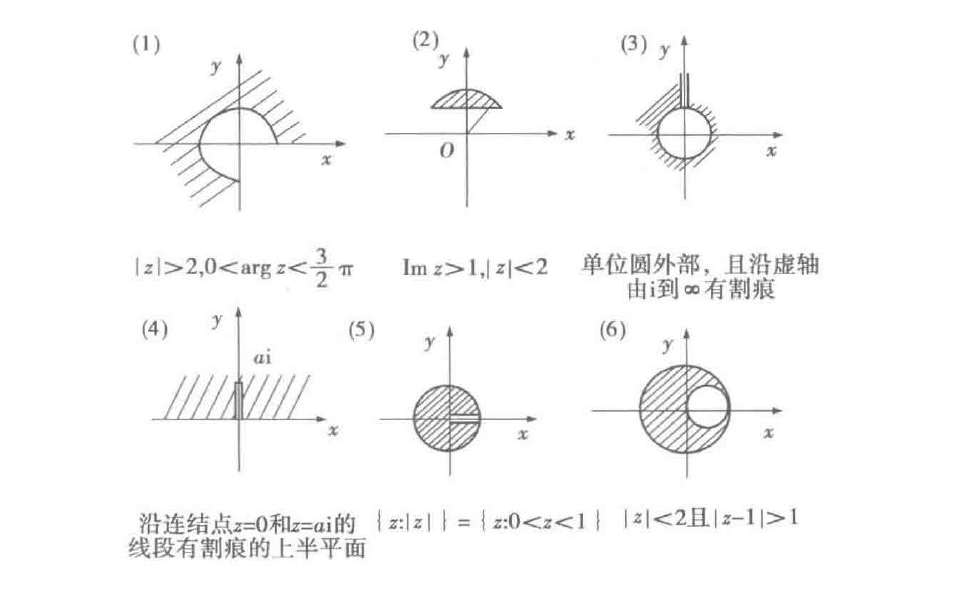
\includegraphics[width=0.92\textwidth]{figures/图6-25.png}
\caption{题 10 所用图（教材图 6.25）}
\label{fig:625}
\end{figure}

\item 设 $w=f(z)$ 是单位圆盘到自身的分式线性映射，证明对于单位圆内任意两点 $z_1,z_2$ 有
\[
\left|\frac{z_1-z_2}{1-\overline{z_1}z_2}\right|
=\left|\frac{w_1-w_2}{1-\overline{w_1}w_2}\right|,
\qquad w_k=f(z_k)\quad(k=1,2).
\]

\item 求出一个把右半平面 $\Ree z>0$ 映射成单位圆 $|w|<1$ 的保形映射。

\item 求出一个单位圆到自身的分式线性映射，使得 $\dfrac12,2$ 为不变点，$(5+3\ii)/4$ 变为无穷远点。

\item 求 $w=\ii\dfrac{z+2}{z-2}$ 将 $|z|>2$ 映射成的区域。

\item 求把 $z$ 平面上的区域 $0<\arg z<\dfrac\pi2$ 映射成 $w$ 平面上的区域 $\Imm w>0$，且把点
$z_1=\sqrt2\ii,z_2=0,z_3=1$ 依次映射成 $w_1=0,w_2=\infty,w_3=-1$ 的保形映射。

\item 试将 $\Imm z>0$ 保形映射成等腰直角三角形，而且使 $z=0,1,\infty$ 分别于 $w=0,a,a+a\ii\ (a>0)$ 相对应。

\item 求把上半 $z$ 平面映射成 $w$ 平面中如图~\ref{fig:626} 所示的阴影部分的保形映射，并使 $x=0$ 对应于 $A$ 点，$x=-1$ 对应于 $B$ 点。

\begin{figure}[H]
\centering
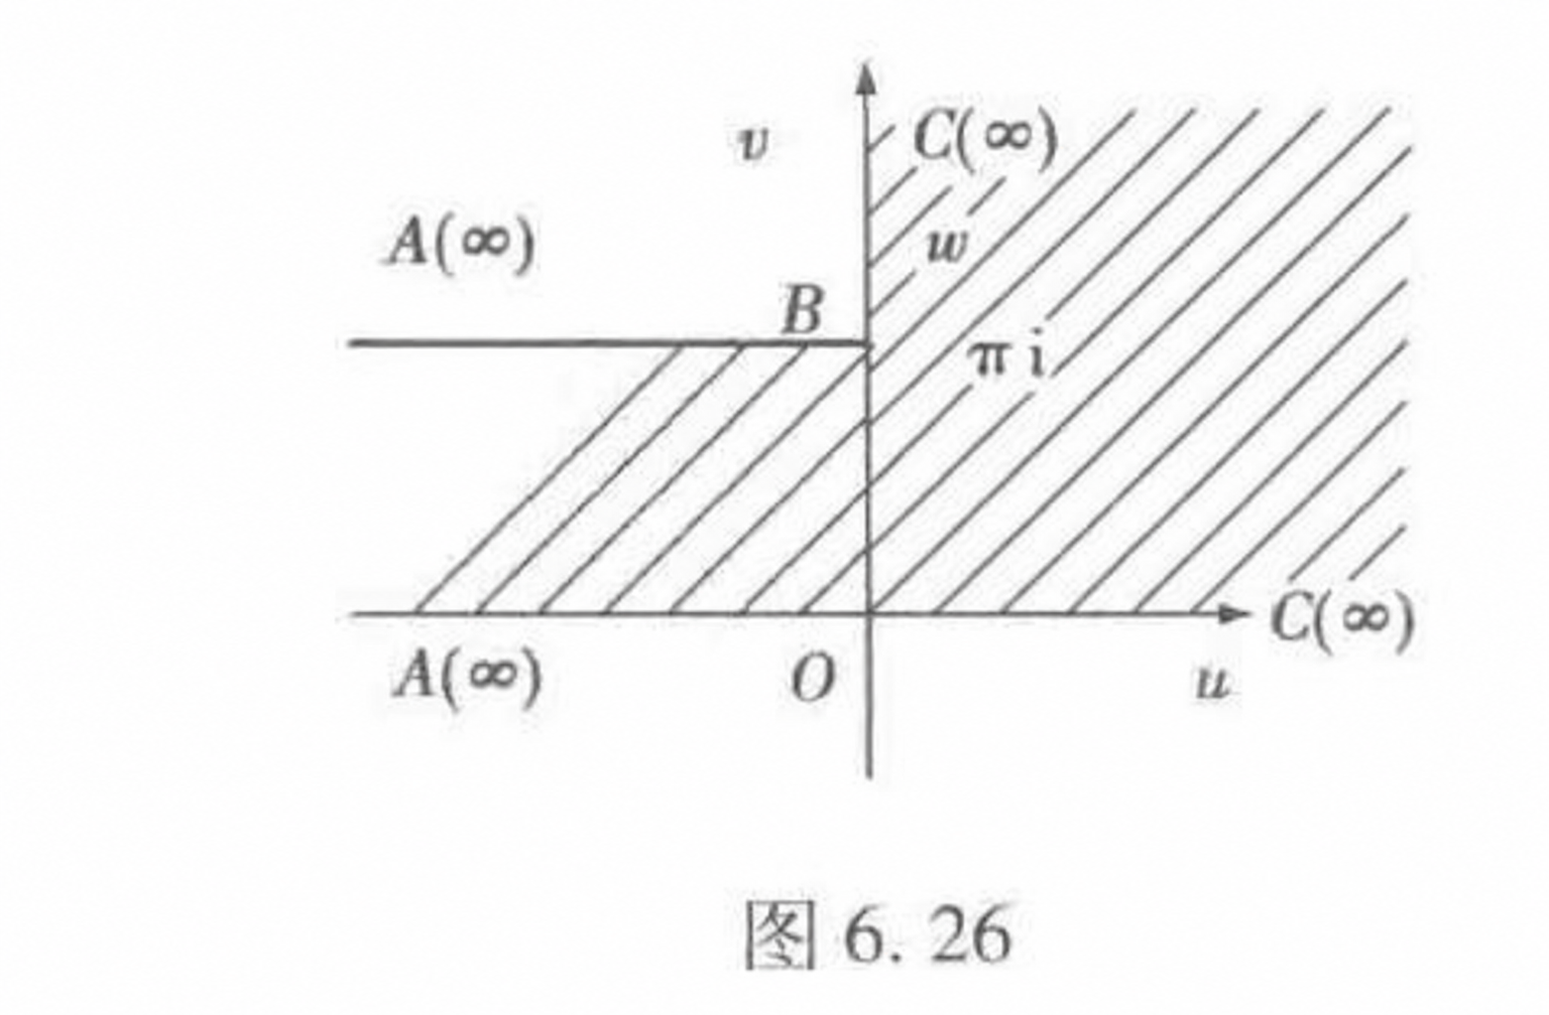
\includegraphics[width=0.58\textwidth]{figures/图6-26_修正版.png}
\caption{题 17 所用图（教材图 6.26）}
\label{fig:626}
\end{figure}

\item 试证明函数
\[
w=\int_0^z\frac{\dd z}{\sqrt{z(1-z^2)}}
\]
将上半平面 $\Imm z>0$ 映射成为一个边长等于
$\dfrac1{2\sqrt{2\pi}}\Gamma^2\!\left(\dfrac14\right)$ 的正方形内部。

\item 试将 $\Imm z>0$ 保形映射成具有锐角 $\pi/6,\pi/3$ 的直角三角形，而且使 $z=0,1,\infty$ 分别与
$w=0,a,a+\dfrac a{\sqrt3}\ii$ 对应（$a>0$）。
\end{enumerate}

% 补充参考：T. A. Driscoll, Schwarz--Christoffel Toolbox User's Guide, §2.1.
% https://citeseerx.ist.psu.edu/document?doi=e1b349f7c2e13ca5903fa87f0e7289e91ecd4adc&repid=rep1&type=pdf
\subsection*{补充：施瓦茨--克里斯托费尔公式}

施瓦茨--克里斯托费尔（Schwarz--Christoffel）公式用于构造上半平面
$\Imm z>0$ 到多边形内部的共形映射。先以具有有限顶点的简单多边形为例：
设按边界正向排列的顶点为 $w_1,\ldots,w_n$，相应内角为
$\alpha_1\pi,\ldots,\alpha_n\pi$，其中 $0<\alpha_j<2$，且
$\sum_{j=1}^n\alpha_j=n-2$。
选择这些顶点在扩充实轴上的原像为
$x_1<x_2<\cdots<x_{n-1}$ 及 $x_n=\infty$，则映射具有形式
\[
\boxed{\displaystyle
w=f(z)=C_0+C_1\int_{z_0}^{z}
\prod_{j=1}^{n-1}(\zeta-x_j)^{\alpha_j-1}\dd\zeta,
\qquad C_1\ne0.}
\]
这里 $z_0$ 是上半平面内的固定基点，积分路径取在上半平面内；各幂函数在该域内
选取一致的解析分支，例如令 $0<\Arg(\zeta-x_j)<\pi$。
常数 $C_0$ 控制平移，$C_1$ 控制伸缩和旋转；原像点 $x_j$ 及这些常数
需由多边形的形状、边长和指定的点对应关系确定。

\noindent\textbf{使用要点：}
每个有限原像点对应的因子，其指数等于“像域在该顶点处的内角除以 $\pi$，再减 $1$”，即
\[
f'(z)=C_1\prod_{j=1}^{n-1}(z-x_j)^{\alpha_j-1},
\qquad
\begin{array}{c|cccc}
\text{内角} & \pi/6 & \pi/3 & \pi/2 & 3\pi/2\\
\hline
\text{指数} & -5/6 & -2/3 & -1/2 & 1/2
\end{array}
\]
当某个顶点的原像选为 $\infty$ 时，乘积中省去该点对应的因子，其角度由映射在无穷远处
的行为体现；不能写成 $(z-\infty)^{\alpha_n-1}$。
例如，三角形的三个顶点原像取为 $0,1,\infty$，对应内角为
$\alpha\pi,\beta\pi,\gamma\pi$，其中 $\alpha+\beta+\gamma=1$，则
\[
w=C_0+C_1\int_{z_0}^{z}
\zeta^{\alpha-1}(\zeta-1)^{\beta-1}\dd\zeta.
\]
对于图 6.26 这类含无穷远顶点的无界多边形，还需结合无穷远处的边界走向，
采用相应的广义内角约定或由有限多边形取极限，不能将无穷远顶点当作普通有限顶点套用内角。


\newpage
\section{习题七：Fourier 变换（P128--P132）}

\begin{enumerate}
\item 求下列函数的傅氏积分表达式。
  \begin{enumerate}
  \item $\displaystyle f(t)=\begin{cases}1-t^2,&|t|<1,\\0,&|t|>1;\end{cases}$
  \item $\displaystyle f(t)=\begin{cases}0,&t<0,\\\ee^{-t}\sin2t,&t\geqslant0;\end{cases}$
  \item $\displaystyle f(t)=\begin{cases}-1,&-1<t<0,\\1,&0<t<1,\\0,&\text{其他。}\end{cases}$
  \end{enumerate}

\item 求证如果 $f(t)$ 满足傅氏积分定理条件，当 $f(t)$ 为奇函数时，则有
\[
f(t)=\int_0^{+\infty}b(\omega)\sin(\omega t)\dd\omega,
\qquad b(\omega)=\frac2\pi\int_0^{+\infty}f(t)\sin(\omega t)\dd t;
\]
当 $f(t)$ 为偶函数时，则有
\[
f(t)=\int_0^{+\infty}a(\omega)\cos(\omega t)\dd\omega,
\qquad a(\omega)=\frac2\pi\int_0^{+\infty}f(t)\cos(\omega t)\dd t.
\]

\item 利用习题 2 的结论，设
$\displaystyle f(t)=\begin{cases}1,&|t|<1,\\0,&|t|>1,
\end{cases}$
试算出 $a(\omega)$，并推证
\[
\int_0^{+\infty}\frac{\sin\omega\cos(\omega t)}{\omega}\dd\omega
=\begin{cases}
\pi/2,&|t|<1,\\
\pi/4,&|t|=1,\\
0,&|t|>1.
\end{cases}
\]

\item 求下列函数的傅里叶变换。
  \begin{enumerate}
  \item $\displaystyle f(t)=\begin{cases}1-|t|,&|t|\leqslant1,\\0,&|t|>1;\end{cases}$
  \item $\displaystyle f(t)=\begin{cases}E,&0\leqslant t\leqslant\tau,\\0,&\text{其他，}\end{cases}\quad(E,\tau>0)$；
  \item $\displaystyle f(t)=\begin{cases}\ee^{-|t|},&|t|<1/2,\\0,&|t|>1/2;\end{cases}$
  \item $\displaystyle f(t)=\frac1{\sqrt{2\pi}\sigma}\ee^{-t^2/(2\sigma^2)}$（此函数称为高斯（Gauss）分布函数）。
  \end{enumerate}

\item 求下列函数的傅里叶变换，并推证下列积分结果。
  \begin{enumerate}
  \item $f(t)=\ee^{-|t|}\cos t$，证明
  \[
  \int_0^{+\infty}\frac{\omega^2+2}{\omega^4+4}\cos(\omega t)\dd\omega
  =\frac\pi2\ee^{-|t|}\cos t.
  \]
  \item $\displaystyle f(t)=\begin{cases}\sin t,&|t|\leqslant\pi,\\0,&|t|>\pi,
  \end{cases}$ 证明
  \[
  \int_0^{+\infty}\frac{\sin(\omega\pi)\sin(\omega t)}{1-\omega^2}\dd\omega
  =\begin{cases}\dfrac\pi2\sin t,&|t|\leqslant\pi,\\0,&|t|>\pi.\end{cases}
  \]
  \end{enumerate}

\item 计算下列积分。
  \begin{enumerate}
  \item $\displaystyle\int_{-\infty}^{+\infty}\delta(t)\sin(\omega_0t)f(t)\dd t$；
  \item $\displaystyle\int_{-\infty}^{+\infty}\delta(t)\cos(\omega_0t)f(t)\dd t$；
  \item $\displaystyle\int_{-\infty}^{+\infty}\delta(t-3)(t^2+1)\dd t$；
  \item $\displaystyle\int_{-\infty}^{+\infty}\delta''\!\left(t-\frac\pi4\right)\sin t\dd t$。
  \end{enumerate}

\item 求下列函数的傅氏变换，其中 $H(t)$ 为 Heaviside 函数。
  \begin{enumerate}
  \item $f(t)=H(t)\sin(\omega_0t)$；
  \item $f(t)=H(t)\cos(\omega_0t)$；
  \item $f(t)=H(t-\tau)$；
  \item $\displaystyle f(t)=\frac12\left[\delta(t+t_0)+\delta(t-t_0)+\delta\left(t+\frac{t_0}{2}\right)+\delta\left(t-\frac{t_0}{2}\right)\right]$；
  \item $f(t)=\cos t\sin t$；
  \item $\displaystyle f(t)=\begin{cases}\ee^{-at},&t>0,\\\ee^{at},&t<0,
  \end{cases}\quad(a>0)$。
  \end{enumerate}

\item 试利用傅氏变换的性质求下列函数的傅氏变换。
  \begin{enumerate}
  \item $\displaystyle f_1(t)=\begin{cases}E,&|t|<2,\\0,&|t|\geqslant2,
  \end{cases}\quad
  f_2(t)=\begin{cases}-E,&|t|<1,\\0,&|t|\geqslant1,
  \end{cases}\quad E>0$，$f(t)=3f_1(t)+4f_2(t)$；
  \item $\displaystyle f(t)=\frac{\alpha^2}{\alpha^2+4(\pi t)^2}$；
  \item $\displaystyle f(t)=\ee^{-(\pi t)^2/\alpha}$；
  \item $f(t)=E\delta(t-t_0)$；
  \item $(t-2)f(-2t)$；
  \item $f(2t-5)$。
  \end{enumerate}

\item 利用能量积分公式，求下列积分的值。
  \begin{enumerate}
  \item $\displaystyle\int_{-\infty}^{+\infty}\frac{1-\cos t}{t^2}\dd t$；
  \item $\displaystyle\int_{-\infty}^{+\infty}\left(\frac{1-\cos t}{t}\right)^2\dd t$；
  \item $\displaystyle\int_{-\infty}^{+\infty}\frac{t^2}{(1+t^2)^2}\dd t$；
  \item $\displaystyle\int_{-\infty}^{+\infty}\frac{\sin^4t}{t^2}\dd t$。
  \end{enumerate}

\item 求下列函数的傅氏变换。
  \begin{enumerate}
  \item $f(t)=\ee^{-\alpha t}H(t)\sin\omega_0t\quad(\alpha>0)$；
  \item $f(t)=\ee^{-\alpha t}H(t)\cos\omega_0t\quad(\alpha>0)$；
  \item $f(t)=\ee^{\ii\omega_0t}H(t-t_0)$。
  \end{enumerate}

\item 求下列函数 $f_1(t)$ 与 $f_2(t)$ 的卷积。
  \begin{enumerate}
  \item $f_1(t)=H(t),\ f_2(t)=\ee^{-at}H(t)$；
  \item $f_1(t)=\ee^{-at}H(t),\ f_2(t)=\sin t\cdot u(t)$；
  \item $\displaystyle f_1(t)=\ee^{-t}H(t),\quad
  f_2(t)=\begin{cases}\sin t,&0<t<\dfrac\pi2,\\0,&\text{其他。}\end{cases}$
  \end{enumerate}

\item 设 $\displaystyle\varphi_\lambda(t)=\frac1\pi\frac{\lambda}{t^2+\lambda^2}\ (\lambda>0)$，证明
\[
\underset{\lambda\to0^+}{\operatorname{wlim}}\varphi_\lambda(t)=\delta(t)
\qquad(-\infty<t<\infty).
\]

\item 设
\[
\varphi_\lambda(t)=
\begin{cases}
(\lambda r)^{-1}\exp\!\left(-\dfrac{t^2}{\lambda^2-t^2}\right),&|t|<\lambda,\\
0,&|t|\geqslant\lambda,
\end{cases}
\qquad
r=\int_{-1}^{1}\exp\!\left(-\frac{t^2}{1-t^2}\right)\dd t,
\]
证明
\[
\underset{\lambda\to0^+}{\operatorname{wlim}}\varphi_\lambda(t)=\delta(t)
\qquad(-\infty<t<\infty).
\]

\item 设 $f(t)$ 在 $(-\infty,\infty)$ 上连续可微，求证
\[
f(t)\delta'(t-t_0)=f(t_0)\delta'(t-t_0)-f'(t_0)\delta(t-t_0)
\qquad(-\infty<t<\infty).
\]

\item 对于实常数 $a\ne0$，求证
\[
\delta^{(n)}(at)=a^{-n}|a|^{-1}\delta^{(n)}(t).
\]

\item 求证
\[
\int_{-\infty}^{+\infty}\delta^{(n)}(t)\dd t=0,
\qquad n=1,2,3,\ldots.
\]

\item 已知某函数 $f(t)$ 的傅氏变换为
$\displaystyle F(\omega)=\mathcal F[f(t)]=\dfrac{\sin\omega}{\omega}$，求该函数 $f(t)$。

\item 证明：如果 $\mathcal F[\ee^{\ii\varphi(t)}]=F(\omega)$，其中 $\varphi(t)$ 为一实函数，则
\[
\mathcal F[\cos\varphi(t)]=\frac12\left[F(\omega)+\overline{F(-\omega)}\right],
\qquad
\mathcal F[\sin\varphi(t)]=\frac1{2\ii}\left[F(\omega)-\overline{F(-\omega)}\right],
\]
其中 $\overline{F(-\omega)}$ 为 $F(\omega)$ 的共轭函数。

\item 已知 $F(\omega)=\mathcal F[f(t)]$，证明（翻转性质）
$F(-\omega)=\mathcal F[f(-t)]$。

\item 利用对称性求下列函数所对应的 $f(t)$。
  \begin{enumerate}
  \item $F(\omega)=u(\omega+\omega_0)-u(\omega-\omega_0)$；
  \item $\displaystyle F(\omega)=\begin{cases}\omega_0/\pi,&|\omega|<\omega_0,\\0,&\text{其他。}\end{cases}$
  \end{enumerate}

\item 证明下列各式。
  \begin{enumerate}
  \item $\ee^{\alpha t}[f_1(t)*f_2(t)]=[\ee^{\alpha t}f_1(t)]*[\ee^{\alpha t}f_2(t)]$；
  \item $\dfrac\dd{\dd t}[f_1(t)*f_2(t)]=\left(\dfrac{\dd f_1(t)}{\dd t}\right)*f_2(t)=f_1(t)*\left(\dfrac{\dd f_2(t)}{\dd t}\right)$。
  \end{enumerate}

\item 求下列函数的傅氏变换。
  \begin{enumerate}
  \item $f(t)=\ee^{-\alpha t}\cos(\omega_0t)\,u(t)\quad(\alpha>0)$；
  \item $f(t)=\ee^{\ii\omega_0t}\,u(t-t_0)$；
  \item $f(t)=\ee^{\ii\omega_0t}t\,u(t)$。
  \end{enumerate}

\item 已知某波形的相关函数 $R(\tau)=\dfrac12\cos(\omega_0\tau)$（$\omega_0$ 为常数），求这个波形的能量谱密度。

\item 证明周期为 $T$ 的非正弦函数 $f_T(t)$ 的频谱函数为
\[
F(\omega)=2\pi\sum_{n=-\infty}^{\infty}C_n\delta(\omega-n\omega_0),
\]
其中，$C_n$ 为 $f_T(t)$ 的傅氏级数展开式中的系数。

\item 求出 $\displaystyle f(t)=E\frac{\sin\omega_0t}{t}$ 的频谱函数，并画出它的频谱图。

\item 求如图~\ref{fig:sawtooth} 所示的锯齿形波的频谱函数，并画出它的频谱图。

\begin{figure}[H]
\centering
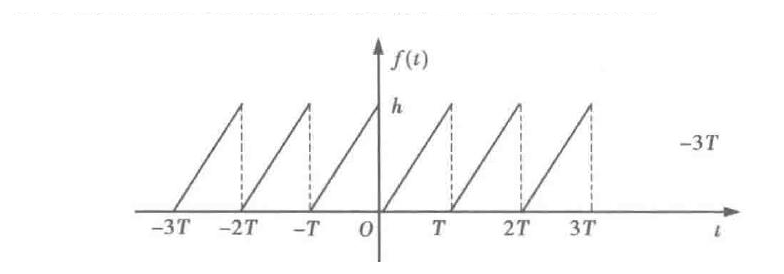
\includegraphics[width=0.72\textwidth]{figures/锯齿形波.png}
\caption{题 26 所用锯齿形波}
\label{fig:sawtooth}
\end{figure}

\item 利用傅氏变换，证明弦振动方程问题
\[
\begin{cases}
\dfrac{\partial^2u}{\partial t^2}=a^2\dfrac{\partial^2u}{\partial x^2},&-\infty<x<+\infty,\ t>0,\\[4pt]
u(x,0)=\varphi(x),\quad
\left.\dfrac{\partial u}{\partial t}\right|_{(x,0)}=\psi(x),&-\infty<x<+\infty
\end{cases}
\]
的解由达朗贝尔（D'Alembert）公式给出：
\[
u(x,t)=\frac12[\varphi(x+at)+\varphi(x-at)]
+\frac1{2a}\int_{x-at}^{x+at}\psi(\tau)\dd\tau.
\]
\end{enumerate}

\newpage
\section{习题八：Laplace 变换（P147--P151）}

\begin{enumerate}
\item 用定义求下列函数的拉氏变换，并用查表的方法来验证结果。
  \begin{enumerate}
  \item $f(t)=\sin\dfrac t3$；
  \item $f(t)=\ee^{-2t}$；
  \item $f(t)=t^2$；
  \item $f(t)=\sin t\cos t$；
  \item $f(t)=\sh kt$；
  \item $f(t)=\cos^2t$。
  \end{enumerate}

\item 求下列函数的拉氏变换。
  \begin{enumerate}
  \item $\displaystyle f(t)=\begin{cases}3,&0\leqslant t<2,\\-1,&2\leqslant t<4,\\0,&t\geqslant4;\end{cases}$
  \item $\displaystyle f(t)=\begin{cases}t+1,&0<t<3,\\0,&t\geqslant3;\end{cases}$
  \item $\displaystyle f(t)=\begin{cases}3,&t<\pi/2,\\\cos t,&t>\pi/2;\end{cases}$
  \item $f(t)=\ee^{2t}+5\delta(t)$；
  \item $f(t)=\delta(t)\cos t-u(t)\sin t$。
  \end{enumerate}

\item 设 $f(t)$ 是以 $2\pi$ 为周期的函数，且在一个周期内的表达式为
\[
f(t)=\begin{cases}\sin t,&0<t\leqslant\pi,\\0,&\pi<t<2\pi,
\end{cases}
\]
求 $\mathcal L[f(t)]$。

\item 求下列函数的拉氏变换式。
  \begin{enumerate}
  \item $f(t)=3t^4-2t^{3/2}+6$；
  \item $f(t)=1-t\ee^t$；
  \item $f(t)=3\sqrt[3]t+4\ee^{2t}$；
  \item $f(t)=\dfrac t{2a}\sin at$；
  \item $f(t)=\dfrac{\sin at}{t}$；
  \item $f(t)=5\sin2t-3\cos2t$；
  \item $f(t)=\ee^{-3t}\cos4t$；
  \item $f(t)=\ee^{-2t}\sin6t$；
  \item $f(t)=t^n\ee^{at}$（$n$ 为整数）；
  \item $f(t)=u(3t-5)$；
  \item $f(t)=\dfrac{\ee^{3t}}{\sqrt t}$；
  \item $f(t)=u(1-\ee^{-t})$。
  \end{enumerate}

\item 利用象函数的导数公式计算下列各式。
  \begin{enumerate}
  \item $f(t)=t\ee^{-3t}\sin2t$，求 $F(s)$；
  \item $\displaystyle f(t)=t\int_0^t\ee^{-3\tau}\sin2\tau\dd\tau$，求 $F(s)$；
  \item $\displaystyle f(t)=\int_0^t\tau\ee^{-3\tau}\sin2\tau\dd\tau$，求 $F(s)$。
  \end{enumerate}

\item 利用象函数的积分公式计算下列各式。
  \begin{enumerate}
  \item $\dfrac{1-\ee^{-t}}t$，求 $F(s)$；
  \item $\dfrac{\ee^{-3t}\sin2t}{t}$，求 $F(s)$；
  \item $\displaystyle\int_0^t\frac{\ee^{-3\tau}\sin2\tau}{\tau}\dd\tau$，求 $F(s)$；
  \item $\dfrac{s}{(s^2-1)^2}$，求 $f(t)$。
  \end{enumerate}

\item 利用拉氏变换的性质求下列函数的拉氏变换。
  \begin{enumerate}
  \item $f(t)=\dfrac{\ee^{bt}-\ee^{at}}t$；
  \item $f(t)=t^2\sin2t$；
  \item $f(t)=\sin\omega t-\omega t\cos\omega t$；
  \item $f(t)=t\sh\omega t$。
  \end{enumerate}

\item 求下列函数的拉氏逆变换。
  \begin{enumerate}
  \item $F(s)=\dfrac1{s^2+4}$；
  \item $F(s)=\dfrac1{s^4}$；
  \item $F(s)=\dfrac1{(s+1)^4}$；
  \item $F(s)=\dfrac1{s+3}$；
  \item $F(s)=\dfrac{2s+3}{s^2+9}$；
  \item $F(s)=\dfrac{s+3}{(s+1)(s-3)}$；
  \item $F(s)=\dfrac{s+1}{s^2+s-6}$；
  \item $F(s)=\dfrac{2s+5}{s^2+4s+13}$。
  \end{enumerate}

\item 设 $f_1(t),f_2(t)$ 均满足拉氏变换存在定理的条件（若它们的增长指数均为 $c_0$），且
$\mathcal L[f_1(t)]=F_1(s)$，$\mathcal L[f_2(t)]=F_2(s)$，则乘积 $f_1(t)f_2(t)$ 的拉氏变换一定存在，且
\[
\mathcal L[f_1(t)f_2(t)]=\frac1{2\pi\ii}
\int_{\beta-\ii\infty}^{\beta+\ii\infty}F_1(q)F_2(s-q)\dd q,
\]
其中 $\beta>0,\Ree s>\beta+c_0$。

\item 求下列函数的拉氏逆变换（象原函数），并用另一种方法加以验证。
  \begin{enumerate}
  \item $F(s)=\dfrac1{s^2+a^2}$；
  \item $F(s)=\dfrac{s}{(s-a)(s-b)}$；
  \item $F(s)=\dfrac{s+c}{(s+a)(s+b)^2}$；
  \item $F(s)=\dfrac{s^2+2a^2}{(s^2+a^2)^2}$；
  \item $F(s)=\dfrac1{(s^2+a^2)s^3}$；
  \item $F(s)=\dfrac1{s(s+a)(s+b)}$；
  \item $F(s)=\dfrac1{s^4-a^4}$；
  \item $F(s)=\dfrac{s^2+2s-1}{s(s-1)^2}$；
  \item $F(s)=\dfrac1{s^2(s^2-1)}$；
  \item $F(s)=\dfrac{s}{(s^2+1)(s^2+4)}$。
  \end{enumerate}

\item 求下列函数的拉氏逆变换。
  \begin{enumerate}
  \item $F(s)=\dfrac1{(s^2+4)^2}$；
  \item $F(s)=\dfrac s{s+2}$；
  \item $F(s)=\dfrac{2s+1}{s(s+1)(s+2)}$；
  \item $F(s)=\dfrac1{s^4+5s^2+4}$；
  \item $F(s)=\dfrac{s+1}{9s^2+6s+5}$；
  \item $F(s)=\ln\dfrac{s^2-1}{s^2}$；
  \item $F(s)=\dfrac{s+2}{(s^2+4s+5)^2}$；
  \item $F(s)=\dfrac1{(s^2+2s+2)^2}$；
  \item $F(s)=\dfrac{s^2+4s+4}{(s^2+4s+13)^2}$；
  \item $F(s)=\dfrac{2s^2+s+5}{s^3+6s^2+11s+6}$；
  \item $F(s)=\dfrac{s+3}{s^3+3s^2+6s+4}$；
  \item $F(s)=\dfrac{2s^2+3s+3}{(s+1)(s+3)^3}$；
  \item $F(s)=\dfrac{1+\ee^{-2s}}{s^2}$；
  \item $F(s)=\dfrac{2s^3+10s^2+8s+40}{s^2(s^2+9)}$；
  \item $F(s)=\dfrac{s^2-3}{(s+2)(s-3)(s^2+2s+5)}$；
  \item $F(s)=\dfrac{2s^3-s^2-1}{(s+1)^2(s^2+1)^2}$。
  \end{enumerate}

\item 试求下列微分方程或微分方程组初值问题的解。
  \begin{enumerate}
  \item $x''+k^2x=0,\quad x(0)=A,\ x'(0)=B$；
  \item $x''+4x'+3x=\ee^{-t},\quad x(0)=x'(0)=1$；
  \item $x''+k^2x=a[u(t)-u(t-b)],\quad x(0)=x'(0)=0$；
  \item $x''-x=4\sin t+5\cos2t,\quad x(0)=-1,\ x'(0)=-2$；
  \item $x^{(4)}+2x'''-2x'-x=\delta(t),\quad x(0)=x'(0)=x''(0)=x'''(0)=0$；
  \item $x^{(4)}+2x''+x=\sin t,\quad x(0)=1,\ x'(0)=-2,\ x''(0)=3,\ x'''(0)=0$；
  \item $x''+4x'+5x=f(t),\quad x(0)=c_1,\ x'(0)=c_2$；
  \item $x'''+x'=\ee^{-2t}+\delta(t)+\delta(t-1),\quad x(0)=x'(0)=x''(0)=0$；
  \item $x''+4x'+5x=\delta(t)+\delta'(t),\quad x(0)=0,\ x'(0)=2$；
  \item $x^{(4)}+x'''=3\delta(t)+u(t-1)+\cos t,\quad x(0)=x'(0)=x'''(0)=0,\ x''(0)=c$（常数）；
  \item $\displaystyle\begin{cases}x'+y'=1+\delta(t),\\x'-y'=t+\delta(t-1),\end{cases}\quad x(0)=a,\ y(0)=b$；
  \item $\displaystyle\begin{cases}x'+x-y=\ee^t,\\3x+y'-2y=2\ee^t,\end{cases}\quad x(0)=y(0)=1$；
  \item $\displaystyle\begin{cases}y'-2z'=f(t),\\y''-z''+z=0,\end{cases}\quad y(0)=y'(0)=z(0)=z'(0)=0$；
  \item $\displaystyle\begin{cases}(2x''-x'+9x)-(y''+y'+3y)=0,\\(2x''+x'+7x)-(y''-y'+5y)=0,
  \end{cases}\quad x(0)=x'(0)=1,\ y(0)=y'(0)=0$；
  \item $\displaystyle\begin{cases}x''-x+y+z=0,\\x+y''-y+z=0,\\x+y+z''-z=0,
  \end{cases}\quad x(0)=1,\ y(0)=z(0)=x'(0)=y'(0)=z'(0)=0$。
  \end{enumerate}

\item 求下列各图所示周期函数的拉氏变换（见图~\ref{fig:periodic}）。

\begin{figure}[H]
\centering
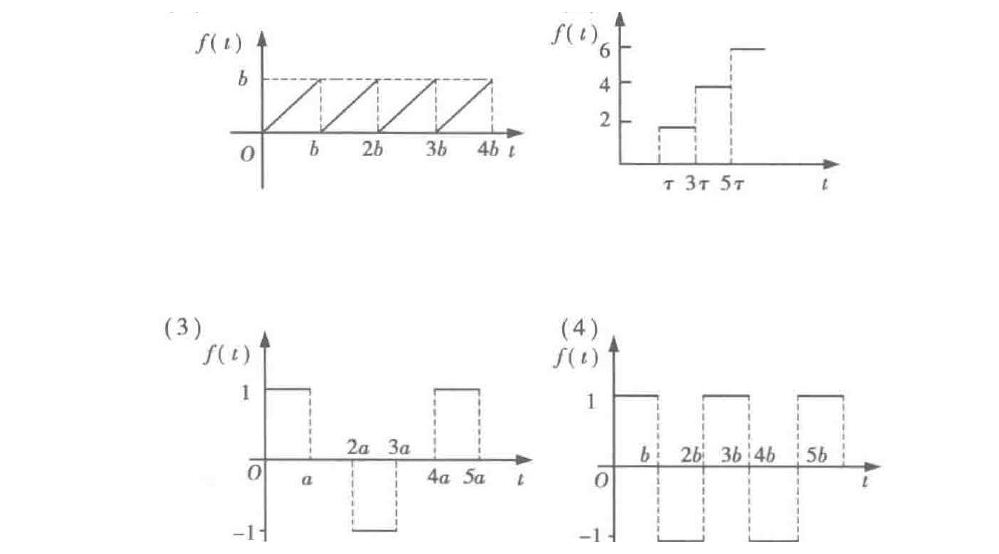
\includegraphics[width=0.9\textwidth]{figures/周期函数.png}
\caption{题 13 所用四个周期函数图像}
\label{fig:periodic}
\end{figure}

\item 计算下列积分。
  \begin{enumerate}
  \item $\displaystyle\int_0^{+\infty}\frac{\ee^{-t}-\ee^{-2t}}t\dd t$；
  \item $\displaystyle\int_0^{+\infty}\frac{1-\cos t}{t}\ee^{-t}\dd t$；
  \item $\displaystyle\int_0^{+\infty}\frac{\ee^{-at}\cos bt-\ee^{-mt}\cos nt}{t}\dd t$；
  \item $\displaystyle\int_0^{+\infty}\ee^{-3t}\cos2t\dd t$；
  \item $\displaystyle\int_0^{+\infty}t\ee^{-2t}\dd t$；
  \item $\displaystyle\int_0^{+\infty}t\ee^{-3t}\sin2t\dd t$；
  \item $\displaystyle\int_0^{+\infty}\frac{\ee^{-\sqrt2t}\sh t\cdot\sin t}{t}\dd t$；
  \item $\displaystyle\int_0^{+\infty}\frac{\ee^{-t}\sin^2t}{t}\dd t$；
  \item $\displaystyle\int_0^{+\infty}t^3\ee^{-t}\sin t\dd t$；
  \item $\displaystyle\int_0^{+\infty}\frac{\sin^2t}{t^2}\dd t$。
  \end{enumerate}

\item 求下列卷积。
  \begin{enumerate}
  \item $1*1$；
  \item $t*t$；
  \item $t^m*t^n$（$m,n$ 为正整数）；
  \item $t*\ee^t$；
  \item $\sin t*\cos t$；
  \item $\sin kt*\sin kt$；
  \item $t*\sh t$；
  \item $\sh at*\sh at$；
  \item $u(t-a)*f(t)$；
  \item $\delta(t-a)*f(t)$。
  \end{enumerate}

\item 利用卷积定理证明
\[
\mathcal L^{-1}\!\left[\frac{s}{(s^2+a^2)^2}\right]=\frac t{2a}\sin at.
\]

\item 利用卷积定理证明
\[
\mathcal L^{-1}\!\left[\frac1{\sqrt s(s-1)}\right]
=\frac2{\sqrt\pi}\ee^t\int_0^{\sqrt t}\ee^{-\tau^2}\dd\tau,
\]
并求 $\displaystyle\mathcal L^{-1}\!\left[\frac1{s\sqrt{s+1}}\right]$。

\item 试求下列积分方程的解。
  \begin{enumerate}
  \item $\displaystyle y(t)=at+\int_0^t y(\tau)\sin(t-\tau)\dd\tau$；
  \item $\displaystyle y(t)=a\sin bt+c\int_0^t y(\tau)\sin b(t-\tau)\dd\tau$，其中 $b>c>0$。
  \end{enumerate}

\item 设在原处质量为 $m$ 的一质点在 $t=0$ 时，在 $x$ 方向上受到冲击力 $k\delta(t)$ 的作用，其中 $k$ 为常数，假定质点的初速度为零，求其运动规律。

\item 某系统的传递函数 $H(s)=\dfrac{k}{1+Ts}$，求当激励 $x(t)=A\sin\omega t$ 时的系统响应 $y(t)$。

% 注解参考：University of Michigan, Control Tutorials, Introduction: System Modeling.
% https://ctms.engin.umich.edu/CTMS/index.php?example=Introduction&section=SystemModeling
\par\smallskip
\noindent\textbf{注：什么是传递函数？}
对于线性时不变系统，在\textbf{零初始条件}（系统初始储能或初始状态为零）下，
传递函数是输出与输入的拉普拉斯变换之比：
\[
H(s)=\frac{Y(s)}{X(s)},\qquad
X(s)=\mathcal L[x(t)],\quad Y(s)=\mathcal L[y(t)].
\]
它描述系统怎样把输入（激励）变成输出（响应），由系统本身决定。
已知输入后，可先求 $Y(s)=H(s)X(s)$，再作拉氏逆变换得到 $y(t)$；
这里取比值的是拉氏变换，不能理解成时域中直接计算 $y(t)/x(t)$。

本题按系统初始静止、正弦激励从 $t=0$ 开始作用理解，因而
\[
X(s)=\frac{A\omega}{s^2+\omega^2},\qquad
Y(s)=\frac{kA\omega}{(1+Ts)(s^2+\omega^2)}.
\]
对这个 $Y(s)$ 求逆变换即可得到所求的零状态响应。
等价地，本题的输入输出满足 $T y'(t)+y(t)=k x(t)$，并取 $y(0)=0$。
若初始状态非零，还需另计初始状态引起的响应，仅凭 $Y(s)=H(s)X(s)$ 不能得到总响应。
\end{enumerate}

\newpage

\end{document}
